\documentclass[12pt]{article}
\usepackage{setspace,graphicx,amsmath,geometry,fontspec,titlesec,soul,bm,subfigure}
\titleformat{\section}[block]{\LARGE\bfseries}{\arabic{section}}{1em}{}[]
\titleformat{\subsection}[block]{\Large\bfseries\mdseries}{\arabic{section}.\arabic{subsection}}{1em}{}[]
\titleformat{\subsubsection}[block]{\normalsize\bfseries}{\arabic{subsection}-\alph{subsubsection}}{1em}{}[]
\titleformat{\paragraph}[block]{\small\bfseries}{[\arabic{paragraph}]}{1em}{}[]
\setmainfont{Times New Roman}
\renewcommand{\baselinestretch}{1.15}
\renewcommand\contentsname{Inhaltverzeichnis}
\geometry{a4paper,left=2.5cm,right=2.5cm,top=2.5cm,bottom=2.5cm}
\begin{document}
	\newpagestyle{main}{            
		\sethead{Gruppe 3}{Ingenieurgeodäsie Übung 4}{}     
		\setfoot{}{\thepage}{}     
		\headrule                                     
		\footrule                                       
	}
	\pagestyle{main}
\tableofcontents
\newpage
\section{Einleitung}
Manche Absteckung findet in Tunnel statt, wo Richtungswinkel schwierig bestimmt werden kann. Deshalb ist die Bestimmung der Richtungswinkel durch Vermessungskreisel notwendig \newline
\newline
Diese Übung findet in Messkeller statt, der Richtungswinkel zwischen einem Standpunkt und einer Zielmarke soll bestimmt werden. Dazu ist die Zielmarke einzumessen und die Nordrichtung mit einem Vermessungskreisel zu bestimmen. 
\section{Messkonzepte und Durchführung}
\subsection{Messkonzepte}
Kreisel weist aufgrund der Rotation um die eigene Achse einen Drehimpuls auf, unter Wirkung der Erdrotation wirkt die Schwerkraft als äußere Kraft auf die Rotationsachse des Kreisels. Kreisel verschwenkt seine Rotationsebene und weicht der einwirkenden Kraft rechtwinklig aus. Die Präzessionsbewegung sorgt für Ausrichtung der Kreiselachse nach Norden. \newline
Gesamtdrehmoment:
\begin{equation*}
D = I_w \cdot \omega_E \cos \varphi \sin A
\end{equation*}
wobei $I_w$ Drehimpuls, $\omega_E$ Erdrotationswinkelgeschwindigkeit, $\varphi$ Breite und $A$ Auslenkung sind.
\subsection{Durchführung}
Um die Nord-Richtung zu bestimmen, sind folgende Schritte durchzuführen: 
\subsubsection{Bestimmung des Fehlwinkels}
Ein ziel wird mit dem Tachymeterfernrohr in 2 Lagen angezielt. Danach wird das Ziel mit Kreiselfernrohr angezielt: $\alpha = R_T - R_K$
\subsubsection{Bestimmung der Bandnulllage}
Der Zielpunkt wird mittels des Kreisels angezielt. Die Arretierung des ausgeschalteten Kreisels wird gelöst und der Zeiger durch die Kabelfernbedienung ins Anzeigefeld des Kreisels gebremst. Jetzt können die Umkehrpunkte des Bands im Anzeigefeld angelesen und dokumentiert werden.
\subsubsection{Schnellorientierung}
In dieser Schritt ist die Grobrichtung von Nord zu bestimmen. Der Lichtzeiger wird auf der Skalarmitte durch Drehung der Tachymeteroberbau bis zu den Umkehrpunkte $v_w$ und $v_e$, die Teilkreisel wird jeweils abgelesen: $A_W$ und $A_E$, $N = \frac{A_W + A_E}{2}$, Dann macht man die Einstellung von $N$ am Tachymeter für Feinorientierungsmethoden.
\subsubsection{Umkehrpunktmethode}
Dieser Schritt dient als Feinorientierung und ist in 2 Teile durchgeführt
\paragraph{mit nachführen}
\noindent 1. Drehe der Alhidude führt zu Holten des Lichtzeuges in der Skalarmitte.\newline
2. Ablesen des Teilkreises an den Umkehrpunkten \newline
3. Aus jeweils 3 Messungen das Schulen-Mittel bilden. 
\begin{figure*}[ht]\centering
	\subfigure[Umkehrpunktmethode]{
		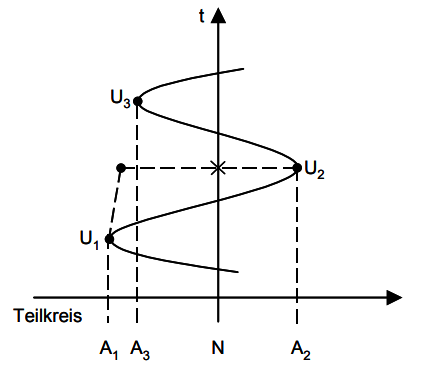
\includegraphics[width=0.9\textwidth]{Umkehrpunktmethode.png}}
\end{figure*}
\paragraph{ohne nachführen}
\noindent 1. Amplitude der Kreisselschwingung dämpfen, bis sich Lichtzeiger nur Gesichtsfeld der Kreiselanzeiger bewegt. \newline
2. Umkehrpunkte an der Hilfsskala ablesen \newline
3. Schule-Mittel und Umrechnung
\subsubsection{Durchgangsmethode}
\begin{figure*}[ht]\centering
	\subfigure[Durchgangsmethode]{
		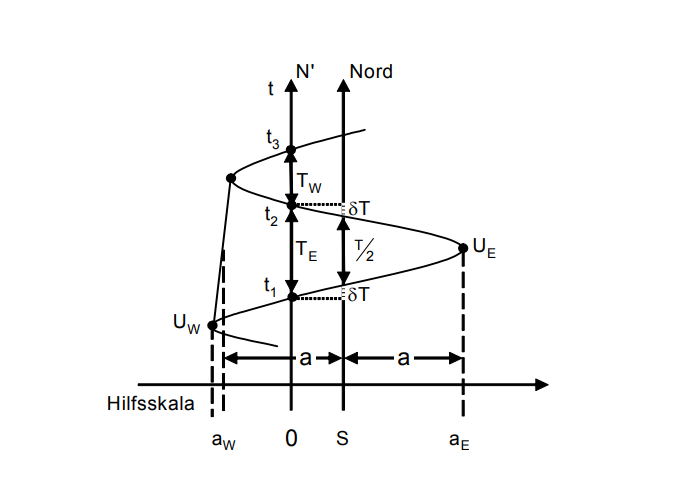
\includegraphics[width=0.9\textwidth]{Durchgangsmethode.png}}
\end{figure*}
1. Voriertierung nd Abbremsen wie in 2-d ohne nachführen. \newline
2. Messung der Durchgangszeiten $t_1$, $t_2$ mit einer Stopuhr \newline 
3. Zusäthliche Ablesung der Amlituden an der Hilfsskala \newline
\section{Genauigkeiten}
\subsection{Groborientierung}
In Schnellorientierung wird der Unterschied innerhalb $\pm 0,05gon$.
\subsection{Feinorientierung}
Bei Umkehrpunktmethode bei 4 bis 6 Umkehrpunkten und bei Durchgangsmethode bei 4 bis 5 Durchgängen sind Standardabweichung $\sigma_N = 5$ bis $10\ mgon$
\section{Diskussion der Ergebnisse}
Alle Ergebnisse ist im Feldbuch im Anhang: der Fehlwinkel $\alpha = 0.1009\ gon$, die Bandnulllage $t_m = -2.82$, damit rechnet man die Bandkorredtion $c_b = dw_{Ort} \varphi t_m = \frac{dw_e}{\cos \varphi} \cdot t_m = 0,0030 gon$, Gyro Orientierung $U = 85.2008\ gon $, Verbesserung$\Delta U = \frac{S}{c} = -0,125\ gon$, Korrektur nach Durchgangspunktmethode $dk = dt \cdot a \cdot C_{prop}$ wird mittels Durchgangspunktmethode berechnet. Eichwert$E = 0,028 gon$ ist gegeben. Dann gibt es:
\begin{equation*}
N = U + \Delta U +dk + E + c_b - alpha = 72.8101 gon
\end{equation*}
Die Ergebnisse bei Umkehrpunktmethode mit nachführen sind nicht gut weil die Unterschied zwischen 2 Schulermitteln ist ca.$0,5\ gon$, das ist ziemlich groß. Der mögliche Grund ist ein Ablesenfehler. 
\newpage
\section{Wiedervorlage}
\subsection{Meridiankonvergenz}
Geographische Koordinaten Messkeller K1:
\begin{equation*}
\lambda = 9°10'30,4'' \quad \quad \varphi = 48°46'55,8''
\end{equation*}
Meridiankonvergenz
\begin{equation*}
\gamma = (\lambda - \lambda_0) \cdot \sin \varphi = 0,14\ gon
\end{equation*}
\subsection{Durchgangspunktmethode}
\begin{gather*}
N' = 85,2008 - 0,75 = 84,4508 gon \\
\delta T = \frac{(T_E - T_W)}{4} \\
T = T_E + T_W \\
S = a \cdot 2\pi \frac{\delta T}{T} = -0,1054\\
N = N' + c \cdot S = 84.4505\ gon
\end{gather*}
Ablesung $Z = 156,2529 gon$, Gerätekonstante $E = 0,0280\ gon$, Fehlwinkel $\alpha = 0,1009 \ gon$
\begin{gather*}
A = Z - N + E - \alpha = 71,7295\ gon \\
\end{gather*}
\end{document}
